\documentclass[11pt,twocolumn]{article}

\usepackage[utf8]{inputenc}
\usepackage[T1]{fontenc}
\usepackage{amsmath,amssymb}
\usepackage{graphicx}
\usepackage{booktabs}
\usepackage{hyperref}
\usepackage[margin=0.75in]{geometry}
\usepackage{cite}
\usepackage{float}

% Allow more floats per page
\renewcommand{\topfraction}{0.9}
\renewcommand{\bottomfraction}{0.9}
\renewcommand{\textfraction}{0.1}
\renewcommand{\floatpagefraction}{0.7}

\title{DeFX: Guitar Effect Removal via Fine-Tuned\\Hybrid Demucs Source Separation}
\author{Neal Flaherty}
\date{}

\begin{document}
\maketitle

\begin{abstract}
We present DeFX, a method for removing distortion, reverb, delay, and other effects from guitar recordings to recover the original clean (dry) signal. DeFX repurposes a pretrained Hybrid Demucs (HDemucs) music source separation model by selectively unfreezing its later encoder and decoder layers while keeping the early feature extraction layers frozen, and attaching a lightweight learned mixing head that combines the separated sources into a single clean guitar estimate. With the last 3 encoder and 3 decoder layers unfrozen on both the frequency and time paths, approximately half of the model's parameters are trainable. Training data is generated synthetically by processing dry guitar recordings through Neural Amp Modeler (NAM) captures and randomized effect chains. We describe the architecture, training procedure, and data generation pipeline, and discuss the implications of transfer learning from source separation to effect inversion.
\end{abstract}

\section{Introduction}

Guitar recordings are frequently captured with amplifier distortion, reverb, delay, and modulation effects baked into the signal. Recovering the underlying clean guitar---the \emph{dry} signal---from such \emph{wet} recordings is useful for re-amping, remixing, and audio restoration. Unlike source separation, which isolates instruments from a mixture, effect removal must invert nonlinear transformations applied to a single instrument.

Recent advances in music source separation, particularly the Hybrid Demucs (HDemucs) architecture \cite{defossez2021hybrid, rouard2023hybrid}, have produced models with strong priors over musical signals. We hypothesize that these priors transfer well to the related task of effect removal, since both problems require understanding the spectral and temporal structure of musical audio.

DeFX exploits this by fine-tuning a pretrained HDemucs model on paired dry/wet guitar audio. We selectively unfreeze the later encoder and decoder layers while keeping the early feature extraction frozen, and learn a mixing head on top, resulting in roughly half of the model's parameters being trainable.

\section{Related Work}

\subsection{Music Source Separation}

Hybrid Demucs \cite{defossez2021hybrid, rouard2023hybrid} combines a temporal convolutional encoder-decoder with a parallel spectrogram-domain transformer branch. Pretrained on the MUSDB18-HQ dataset and additional internal data, it achieves state-of-the-art separation of drums, bass, vocals, and ``other'' sources. We leverage the publicly available \texttt{HDEMUCS\_HIGH\_MUSDB\_PLUS} checkpoint from \texttt{torchaudio}.

\subsection{Neural Amp Modeling}

Neural Amp Modeler (NAM) \cite{nam2023} uses lightweight neural networks (WaveNet, LSTM, or linear architectures) to capture the input-output behavior of guitar amplifiers. Given a set of NAM captures at various amplifier settings, one can process arbitrary dry guitar audio to produce realistic amplified tones. We use NAM captures as the forward model to generate training data for the inverse problem.

\subsection{Audio Effect Removal}

Prior work on effect removal has focused on specific effects such as reverberation \cite{su2020hifi} or distortion in isolation. DeFX addresses the more general problem of removing arbitrary chains of effects, including combinations of amplifier distortion, reverb, delay, chorus, and compression.

\section{Method}

\subsection{Architecture}

DeFX consists of two components: a frozen (or partially unfrozen) HDemucs backbone and a learned mixing head. Figure~\ref{fig:architecture} illustrates the full architecture.

\begin{figure}[htbp]
  \centering
  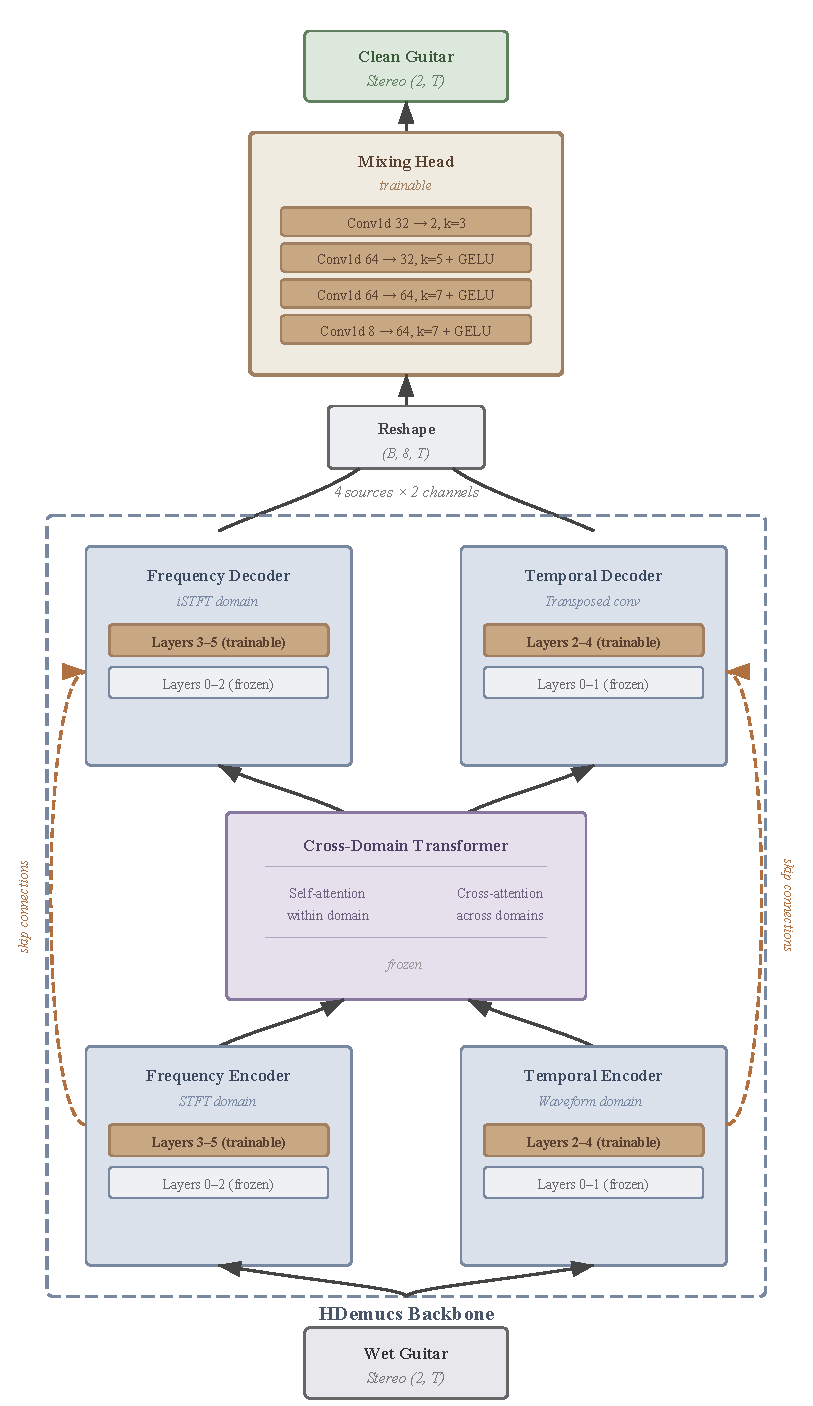
\includegraphics[width=\columnwidth]{figures/architecture.pdf}
  \caption{DeFX architecture. Data flows upward from the wet guitar input through the dual-path HDemucs backbone (frequency and temporal branches with skip connections), then through a learned mixing head that combines the separated sources into a clean stereo output. Shaded layers are trainable; unshaded layers remain frozen.}
  \label{fig:architecture}
\end{figure}

\paragraph{Backbone.} The pretrained HDemucs model was originally trained to separate a song into four stems: drums, bass, vocals, and ``other'' (guitars, keys, synths, etc.). Given a stereo input $\mathbf{x} \in \mathbb{R}^{2 \times T}$, it produces four source estimates $\mathbf{S} \in \mathbb{R}^{4 \times 2 \times T}$. When fed a guitar recording, the ``other'' stem already contains most of the guitar signal, but useful information also appears in the remaining stems---distortion harmonics may be classified as drums, low-end rumble may end up in bass, and so on. We flatten the four stereo sources into a single 8-channel representation $\mathbf{S}' \in \mathbb{R}^{8 \times T}$ to make all of this information available to the mixing head.

\paragraph{Mixing Head.} Rather than simply extracting the ``other'' channel, we use a small 1D convolutional network that learns the optimal way to combine all 8 channels back into a clean stereo guitar signal. The convolution filters slide across the audio, allowing the head to perform operations like ``take mostly the `other' channel but subtract a bit of what ended up in `vocals' to remove a reverb artifact.'' The head consists of four layers:
\begin{align}
\mathbf{h}_1 &= \text{GELU}(\text{Conv1d}_{8 \to 64}^{k=7}(\mathbf{S}')) \\
\mathbf{h}_2 &= \text{GELU}(\text{Conv1d}_{64 \to 64}^{k=7}(\mathbf{h}_1)) \\
\mathbf{h}_3 &= \text{GELU}(\text{Conv1d}_{64 \to 32}^{k=5}(\mathbf{h}_2)) \\
\hat{\mathbf{y}} &= \text{Conv1d}_{32 \to 2}^{k=3}(\mathbf{h}_3)
\end{align}
The first layer expands the 8 source channels to 64 intermediate channels, the middle layers refine the representation, and the final layer compresses it to a 2-channel stereo output.

Critically, the head is initialized to pass through the ``other'' source as-is. Before any training, the model already outputs a reasonable guitar estimate. Training then refines this starting point, which converges much faster than learning from scratch.

\subsection{Selective Unfreezing}

While the mixing head alone provides a useful baseline, selectively unfreezing the later layers of the backbone significantly improves performance. We unfreeze the last 3 layers of both the frequency-domain and time-domain encoder and decoder branches of HDemucs. This results in approximately 44M of the 84M total parameters being trainable ($\sim$52\%), allowing the later layers to adapt to the effect removal task while the frozen early layers retain their general audio feature extraction capabilities.

\subsection{Loss Function}

We train with a composite loss inspired by the L1 loss used in Demucs, augmented with spectral terms:
\begin{equation}
\mathcal{L} = \mathcal{L}_{\text{L1}} + 0.1 \cdot \mathcal{L}_{\text{MRSTFT}} + 0.05 \cdot \mathcal{L}_{\text{Mel}}
\end{equation}
where $\mathcal{L}_{\text{L1}}$ is the mean absolute error in the time domain, $\mathcal{L}_{\text{MRSTFT}}$ is a multi-resolution STFT loss computed at FFT sizes of 512, 1024, and 2048, and $\mathcal{L}_{\text{Mel}}$ is a mel-spectrogram loss with 128 mel bands.

The original Demucs training uses pure L1 loss in the time domain. We retain L1 as the dominant term to preserve waveform fidelity, but add the spectral losses at low weights to encourage perceptually accurate frequency content. In early experiments, we found that weighting the spectral losses more heavily (e.g., equal to L1) produced outputs that, while spectrally accurate, exhibited a hollowed-out quality with audible phasing artifacts. The L1-dominant weighting avoids these issues and produces more natural-sounding results, consistent with the design choice made in the original Demucs training.

\section{Data Generation}

Training data is generated synthetically from the IDMT-SMT-GUITAR\_V2 dataset \cite{idmt2013}, which contains approximately 1{,}173 dry guitar recordings spanning various playing styles and techniques.

\subsection{NAM Amp Pairs}

Each dry recording is processed through a randomly sampled subset of 30 Neural Amp Modeler captures spanning three amplifier types---a Fender-style blackpanel, a Vox-style chime, and a Marshall-style plexi---each at 10 different volume, treble, and bass settings (Table~\ref{tab:nam}). This produces approximately 8{,}000 amp-only wet/dry pairs with diverse tonal characteristics.

\subsection{Effect Chains}

Each dry recording is additionally processed through 14 randomly constructed effect chains, yielding approximately 16{,}000 chain pairs. Chains are sampled from weighted templates including:
\begin{itemize}
\item Amp + reverb (most common)
\item Amp + delay + reverb
\item Amp + chorus + reverb
\item Compressor + amp + reverb
\item Reverb only, delay only, chorus + reverb (no amp)
\item Amp + slapback delay + room reverb
\end{itemize}
Effect parameters (room size, delay time, feedback, mix levels, etc.) are randomized within musically plausible ranges. The effects are implemented using Spotify's Pedalboard library \cite{pedalboard2021}, which provides generic DSP-based audio effects rather than emulations of specific commercial hardware. Approximately 90\% of chains include reverb, reflecting its prevalence in real-world guitar recordings.

\subsection{Passthrough Pairs}

A copy of each dry file is included as a ``passthrough'' pair where the wet signal equals the dry signal. This teaches the model to preserve already-clean signals without introducing artifacts, yielding approximately 1{,}173 additional pairs.

In total, the training set contains approximately 25{,}000 paired examples.

\begin{table}[t]
\centering
\caption{NAM amplifier captures. Three amp types, each captured at 10 gain settings from clean to fully driven. Settings vary slightly per amp to match each amplifier's voicing.}
\label{tab:nam}
\small
\begin{tabular}{@{}ll@{}}
\toprule
Amp Type & Style \\
\midrule
Blackpanel & Fender-style American clean/breakup \\
Chime      & Vox-style British Class A \\
Plexi      & Marshall-style British high gain \\
\bottomrule
\end{tabular}
\vspace{0.5em}

Each amp is captured at 10 settings spanning volume 2.0 (clean) to 10.0 (max drive), with treble and bass varied between 3.0--8.0 to cover bright, neutral, and dark voicings. This yields 30 captures total.
\end{table}

\section{Training}

\subsection{Configuration}

Training uses the AdamW optimizer with a learning rate of $2 \times 10^{-4}$ and cosine annealing to $1\%$ of the initial rate. Batch size is 4, with each sample being a 1-second chunk (44{,}100 samples at 44.1\,kHz) randomly cropped from a training pair. Random gain augmentation between 0.5$\times$ and 1.5$\times$ is applied to both wet and dry signals jointly. Gradient norms are clipped to 1.0.

Training runs for up to 1{,}000 epochs with early stopping triggered after 50 epochs without improvement in training loss. Each epoch is capped at 200 gradient steps to maintain consistent epoch duration regardless of dataset size.

\subsection{Validation}

A 10\% validation split is constructed deterministically by hashing dry filenames, ensuring that all wet variants of a given dry file appear in the same split to prevent data leakage. Validation loss is computed over 50 batches per epoch.

\subsection{Infrastructure}

Training is conducted on AWS SageMaker using a single \texttt{ml.g5.xlarge} instance (NVIDIA A10G GPU, 24\,GB VRAM). Checkpoints are continuously synced to S3, enabling monitoring and recovery from spot instance interruptions.

\section{Results}

We evaluate DeFX on 500 randomly sampled pairs from the held-out validation split (10\% of dry files, deterministically assigned by filename hash). All metrics compare the restored output against the dry ground truth, with the wet input as baseline.

\subsection{Objective Metrics}

Table~\ref{tab:objective} summarizes the objective metrics across all 500 validation pairs. DeFX improves SI-SDR by +4.85\,dB on average, reduces L1 error by 41\%, and cuts mel cepstral distortion by more than half.

\begin{table}[t]
  \centering
  \caption{Objective metrics on the validation set (500 pairs). For SI-SDR, higher is better; for L1, MRSTFT, and MCD, lower is better.}
  \label{tab:objective}
  \begin{tabular}{@{}lrrr@{}}
    \toprule
    Metric & Wet (input) & Restored & $\Delta$ \\
    \midrule
    SI-SDR (dB) $\uparrow$ & $-0.90$ & $3.95$ & $+4.85$ \\
    L1 $\downarrow$ & $0.0298$ & $0.0177$ & $-0.0121$ \\
    MRSTFT $\downarrow$ & $1.934$ & $1.051$ & $-0.883$ \\
    MCD (dB) $\downarrow$ & $95.1$ & $36.2$ & $-58.9$ \\
    \bottomrule
  \end{tabular}
\end{table}

\subsection{Performance by Effect Type}

Figure~\ref{fig:per_effect} shows SI-SDR improvement broken down by effect chain type. The model performs best on chains involving amplifier distortion, with compressor + amp + delay + reverb achieving +10.56\,dB and amp + slapback + room reverb achieving +10.40\,dB. Pure amp distortion removal (amp only and NAM only) yields +8--9\,dB improvement.

Effects-only chains without amplifier distortion are harder to invert: chorus + reverb (+1.56\,dB), delay only (+1.12\,dB), and reverb only ($-0.54$\,dB). This is expected, as the model's training data is dominated by amp-based chains, and time-domain effects like reverb and delay are inherently more difficult to invert due to their long temporal dependencies.

For passthrough pairs (where the input is already clean), the model achieves an absolute SI-SDR of 89\,dB against the ground truth, indicating that it introduces negligible artifacts on unprocessed signals.

\begin{figure}[htbp]
  \centering
  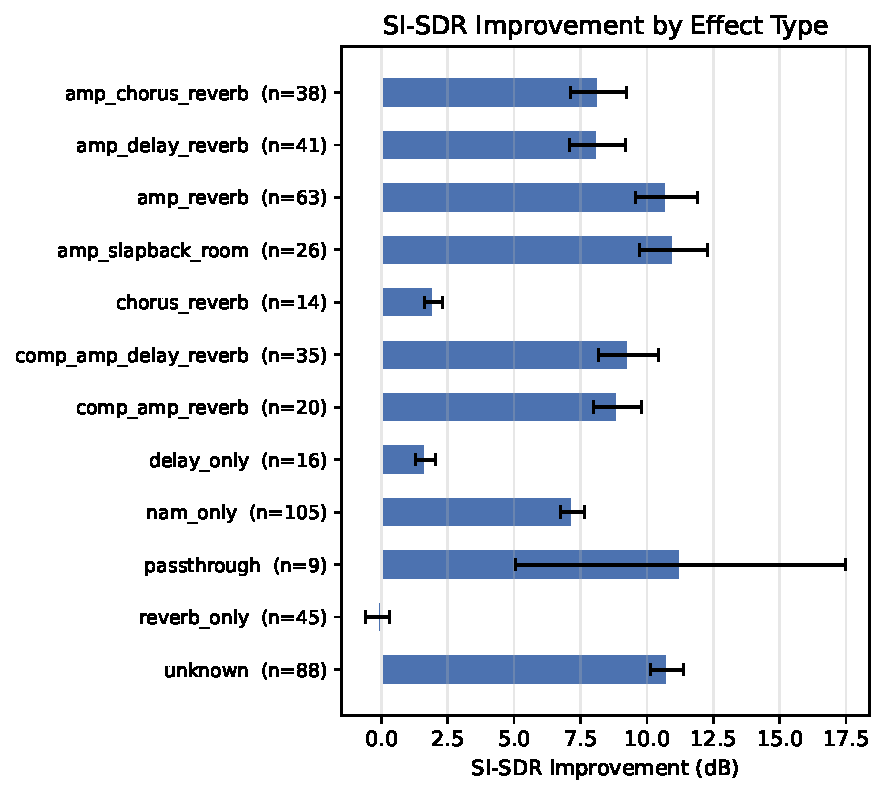
\includegraphics[width=\columnwidth]{figures/per_effect_sisdr.pdf}
  \caption{SI-SDR improvement by effect chain type. Chains involving amplifier distortion show the largest gains. Effects-only chains (reverb, delay, chorus) without amp distortion are harder to remove.}
  \label{fig:per_effect}
\end{figure}

\subsection{Performance by Distortion Level}

Figure~\ref{fig:per_gain} groups results by amplifier gain level. Performance is relatively consistent across all distortion levels: clean (+8.60\,dB), breakup (+7.24\,dB), crunch (+8.22\,dB), and cranked (+7.69\,dB). The model handles heavy distortion nearly as well as light distortion, suggesting that the unfrozen encoder layers learn effective representations across the full gain range.

\begin{figure}[htbp]
  \centering
  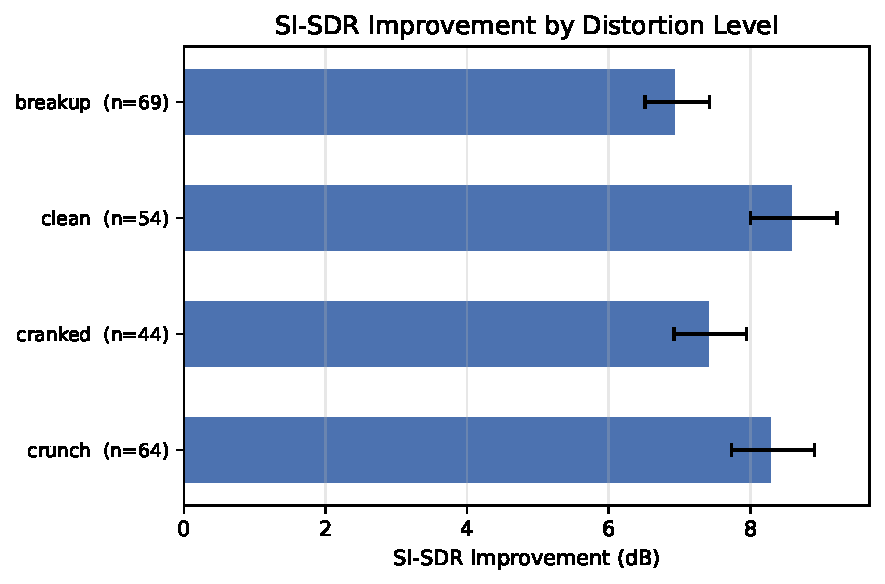
\includegraphics[width=\columnwidth]{figures/per_gain_sisdr.pdf}
  \caption{SI-SDR improvement by amplifier distortion level. Performance is consistent from clean to fully cranked settings.}
  \label{fig:per_gain}
\end{figure}

\subsection{Spectrogram Comparison}

Figure~\ref{fig:spec_nam} shows a representative spectrogram comparison for NAM-only distortion removal. The restored signal closely matches the dry ground truth, with harmonic distortion products visibly reduced.

\begin{figure}[htbp]
  \centering
  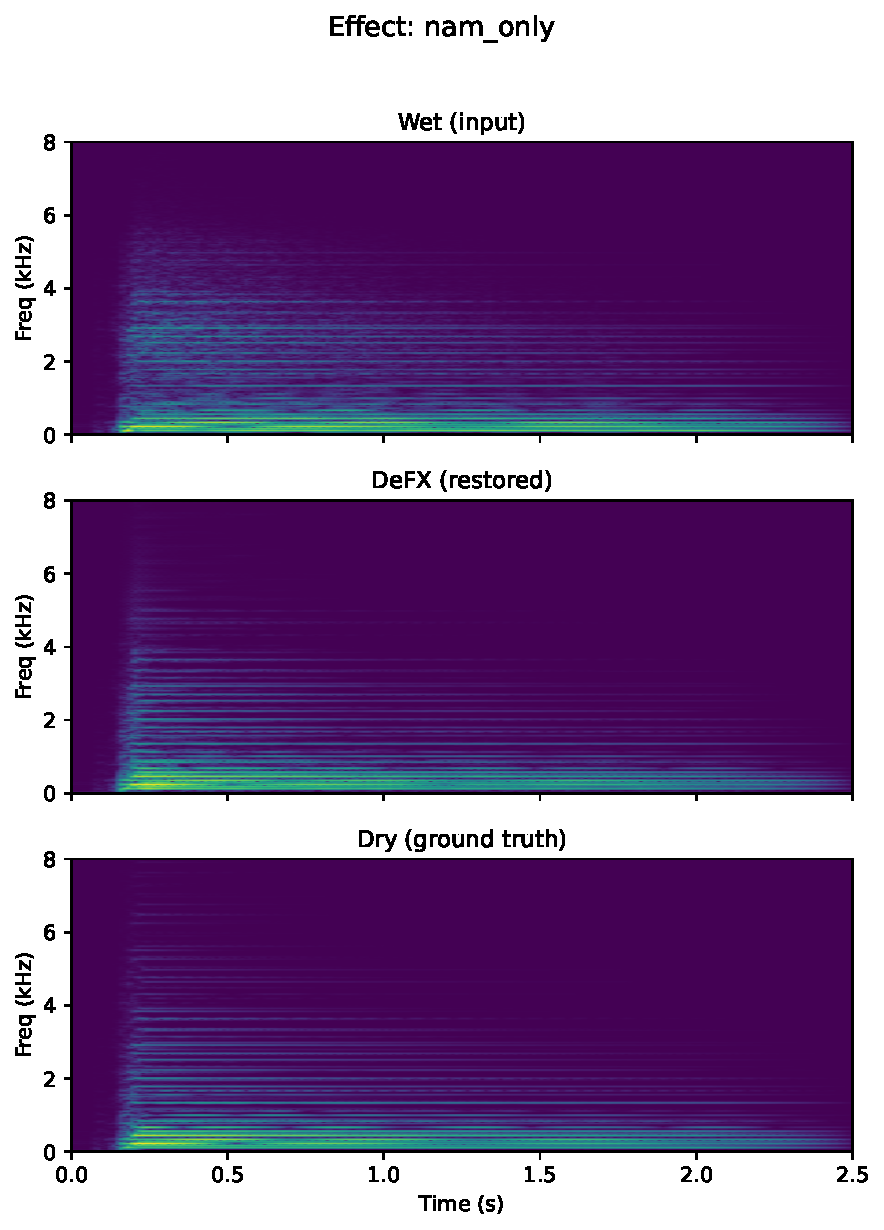
\includegraphics[width=\columnwidth]{figures/spectrogram_nam_only.pdf}
  \caption{Spectrogram comparison for NAM-only distortion: wet input (top), DeFX restored (middle), dry ground truth (bottom). Distortion harmonics are visibly reduced in the restored signal.}
  \label{fig:spec_nam}
\end{figure}

Figure~\ref{fig:spec_chain} shows a more complex case: compressor + amp + delay + reverb. Despite the multiple layered effects, the model recovers much of the original signal structure.

\begin{figure}[htbp]
  \centering
  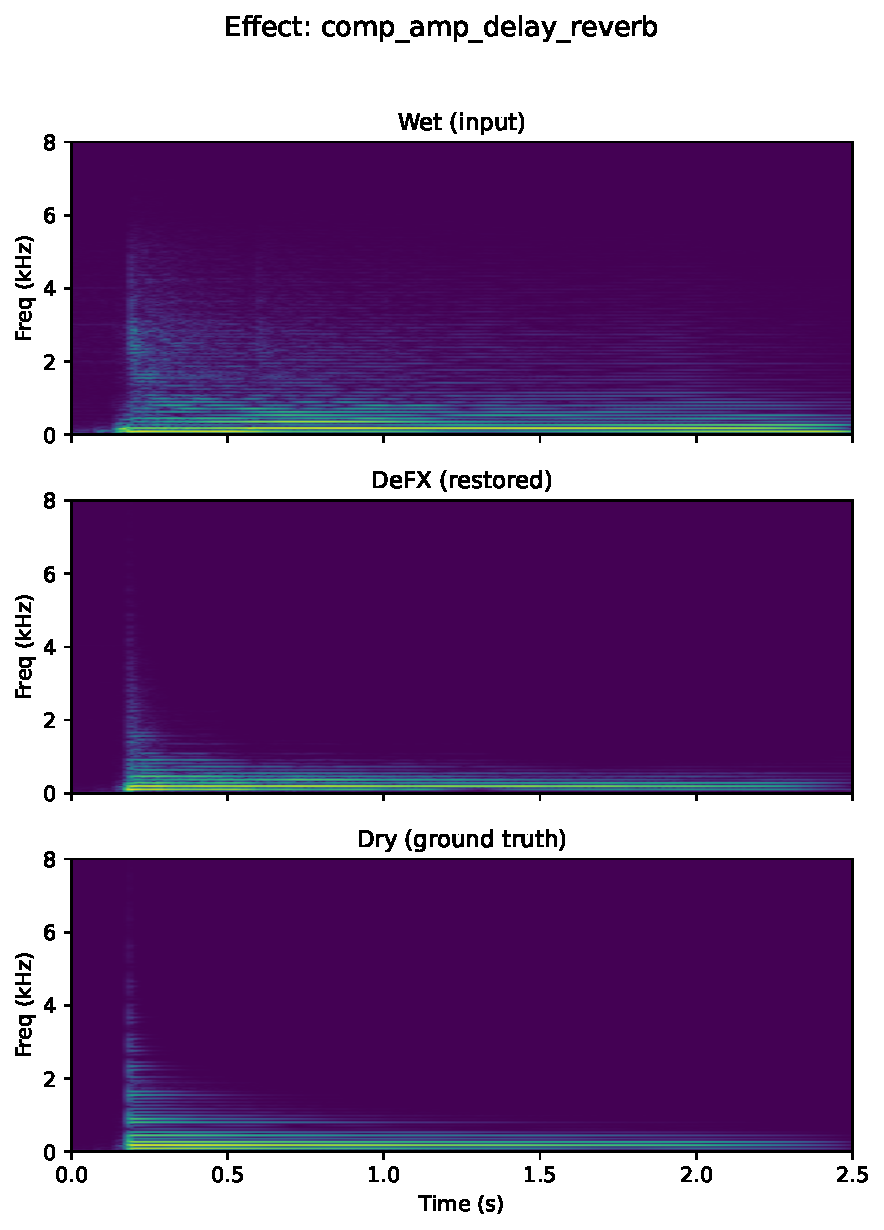
\includegraphics[width=\columnwidth]{figures/spectrogram_comp_amp_delay_reverb.pdf}
  \caption{Spectrogram comparison for compressor + amp + delay + reverb chain: wet input (top), DeFX restored (middle), dry ground truth (bottom).}
  \label{fig:spec_chain}
\end{figure}

\section{Discussion}

\subsection{Transfer Learning from Source Separation}

The key insight of DeFX is that source separation models learn rich representations of musical audio that transfer to effect removal. The HDemucs ``other'' source already captures much of the guitar signal; the mixing head learns to refine this estimate by leveraging information from all four source branches.

\subsection{Head Initialization}

As described in Section 3, the mixing head is initialized to pass through the ``other'' source. This is critical for stable training---without it, the model must simultaneously learn to extract the guitar signal and invert the effects, leading to slower convergence and less stable optimization.

\subsection{Limitations}

DeFX is trained exclusively on guitar audio and may not generalize to other instruments. The synthetic training data, while diverse, does not capture all real-world recording conditions (room acoustics, microphone characteristics, analog circuit behavior). The model operates at 44.1\,kHz and requires input lengths compatible with the HDemucs architecture.

Subjectively, the model handles amplifier distortion well, producing clean and natural-sounding output. However, it struggles with modulation effects such as chorus, where the pitch fluctuations introduced by the effect are difficult to invert. Delay and reverb are noticeably reduced but not fully removed---residual tails and reflections remain audible, particularly for longer delay times and larger reverb spaces. This is consistent with the objective metrics, where effects-only chains (chorus, delay, reverb without amp) show the smallest SI-SDR improvements. These time-domain effects introduce long-range temporal dependencies that are challenging for the model's receptive field to fully capture.

\section{Conclusion}

DeFX demonstrates that pretrained source separation models can be efficiently repurposed for guitar effect removal through selective fine-tuning and a lightweight mixing head. By unfreezing the later encoder and decoder layers while keeping the early feature extraction frozen, roughly half of the backbone adapts to the effect removal task while benefiting from pretrained audio representations. By generating synthetic training data from NAM amplifier captures and randomized effect chains, we avoid the need for expensive paired real-world recordings.

\bibliographystyle{plain}
\begin{thebibliography}{9}

\bibitem{defossez2021hybrid}
A.~D{\'e}fossez.
\newblock Hybrid spectrogram and waveform source separation.
\newblock In \emph{Proc. ISMIR Workshop on Music Source Separation}, 2021.

\bibitem{rouard2023hybrid}
S.~Rouard, F.~Massa, and A.~D{\'e}fossez.
\newblock Hybrid transformers for music source separation.
\newblock In \emph{Proc. IEEE ICASSP}, 2023.

\bibitem{nam2023}
S.~Eichas and S.~M{\"o}ller.
\newblock Neural amp modeler: Neural network emulation of nonlinear audio systems.
\newblock In \emph{Proc. DAFx}, 2023.

\bibitem{idmt2013}
C.~Kehling, J.~Abeßer, C.~Dittmar, and G.~Schuller.
\newblock Automatic tablature transcription of electric guitar recordings by estimation of score- and instrument-related parameters.
\newblock In \emph{Proc. DAFx}, 2014.

\bibitem{su2020hifi}
J.~Su, Z.~Jin, and A.~Finkelstein.
\newblock HiFi-GAN: High-fidelity denoising and dereverberation based on speech deep features in adversarial networks.
\newblock In \emph{Proc. Interspeech}, 2020.

\bibitem{pedalboard2021}
Spotify.
\newblock Pedalboard: A Python library for audio effects.
\newblock \url{https://github.com/spotify/pedalboard}, 2021.

\end{thebibliography}

\end{document}
